\chapter{The Large Hadron Collider}
\label{chap:lhc}

The Standard Model provides a framework for understanding the fundamental particles and the underlying forces which govern their behavior. Among other things, the SM is very successful at modeling scattering amplitudes and decay rates. 

Nature itself has provided us with a source of high-energy particle collisions in the form of cosmic rays. Cosmic rays are very high energy protons and light atomic nuclei which originate from outside the Solar System. When they enter our atmosphere, they collide with the (primarily) nitrogen, oxygen, or argon atoms causing them to break apart creating showers of particles within the atmosphere. As the particles rain down on Earth, many of them decay into less massive ones or are absorbed in the atmosphere - muons and neutrinos are the only particles which make it to the surface. A diagram of this phenomena is seen in Figure \ref{fig:cosmicrays}. Indeed there are many experiments which set out to detect cosmic ray showers, but at the LHC a different approach is taken and we build machines on Earth to generate the particle collisions - although at not nearly such large energies provided by extrastellar space. The particle collisions can be focused to a single part of space, the region around the beam spot can be extensively instrumented to detect the debris of the collision. 

The Large Hadron Collider (LHC) is a facility which houses two beams of protons (each beam centimeters in transverse size) running parallel in an underground ring 17 miles in circumference. The protons are accelerated to nearly the speed of light by electric fields and are steered within their circular trajectory using magnetic fields generated by superconducting magnets. A schematic of the complex which houses this machine is seen in the left panel of Figure \ref{fig:lhc}; as seen in the diagram, the LHC is the final machine of a number of stages which each incrementally increase the energy of the protons. There are 5 locations around the ring where the beams are crossed and particle detectors are placed. The right panel of Figure \ref{fig:lhc} shows the LHC complex underground near Geneva, Switzerland.

\begin{figure}[hb!]
\centering
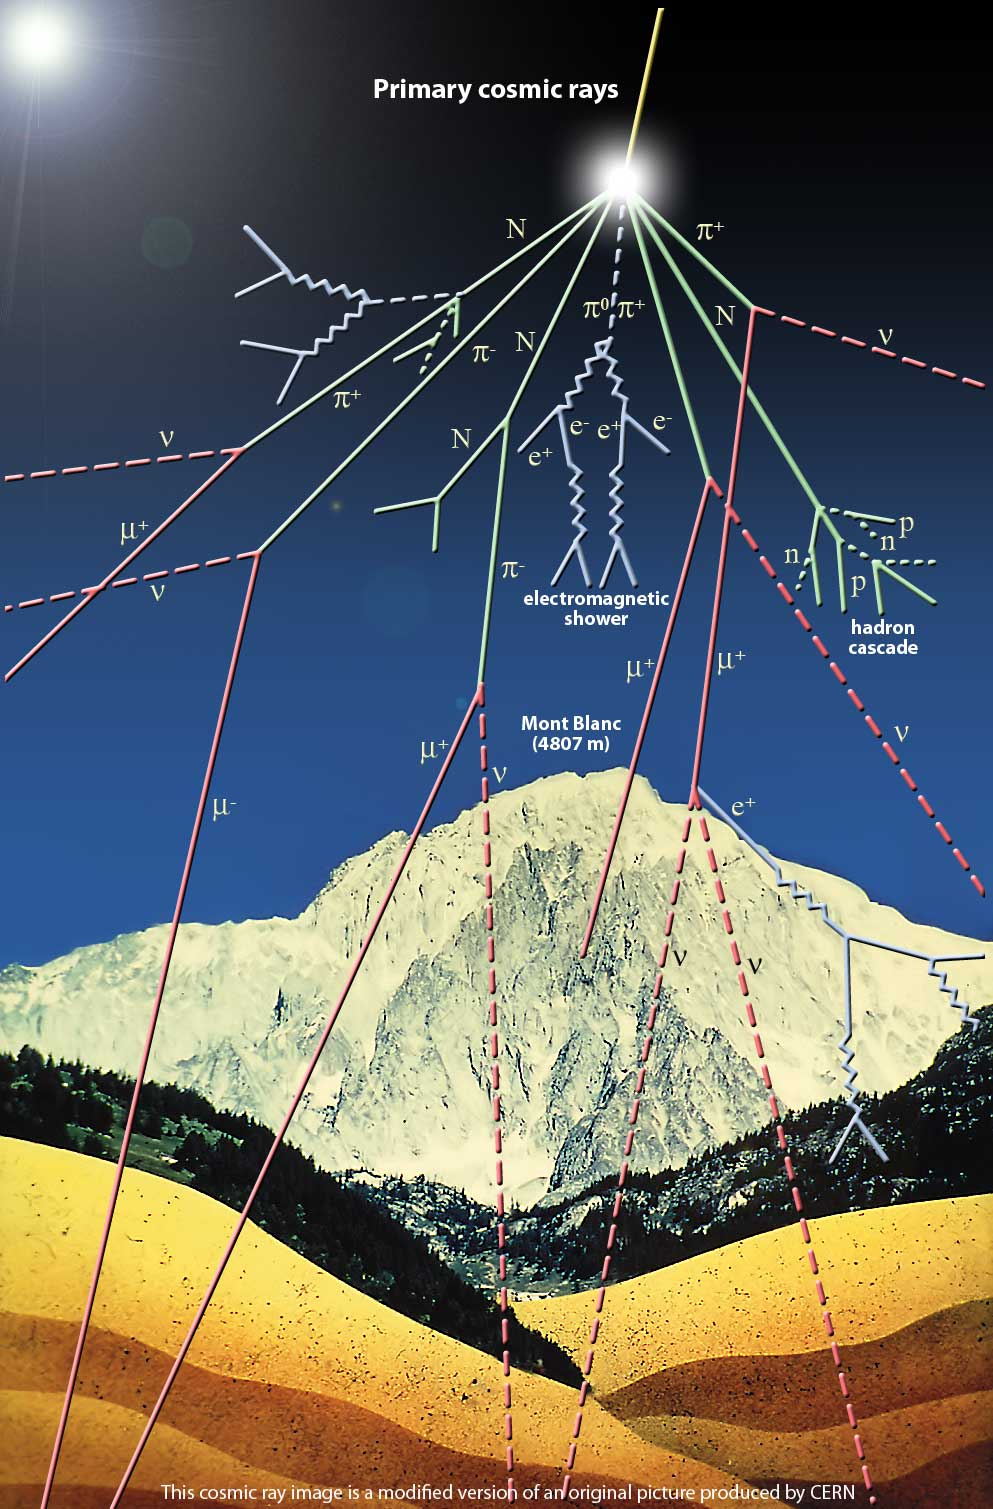
\includegraphics[width=0.45\textwidth]{figs/cosmic-rays.jpg}
\caption{Nature's source of high-energy particle collisions: a cosmic ray shower.}
\label{fig:cosmicrays}
\end{figure}

\begin{figure}[hb!]
\centering
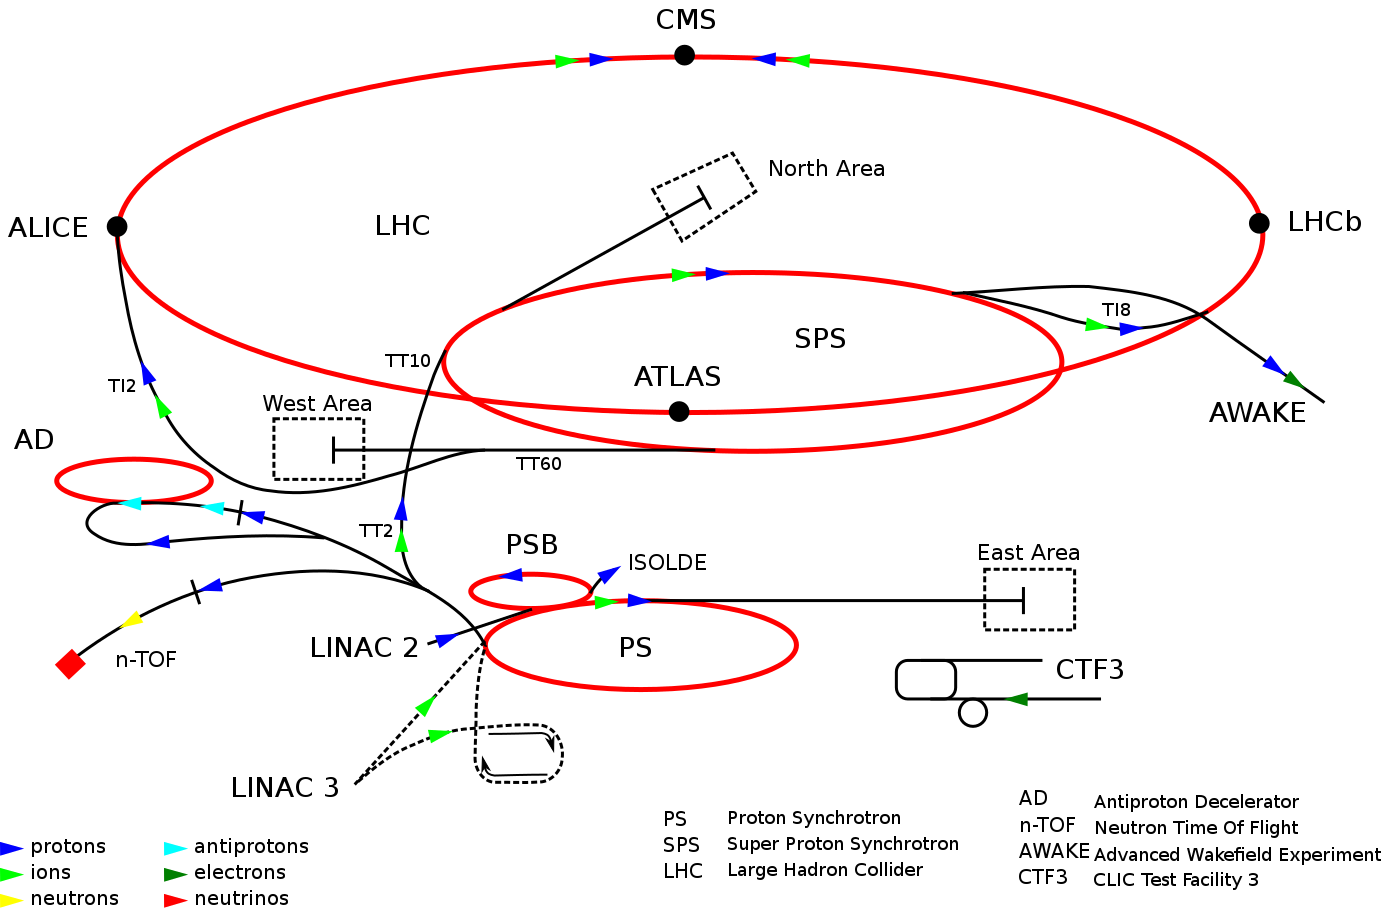
\includegraphics[width=0.55\textwidth]{figs/lhcschematic.png}
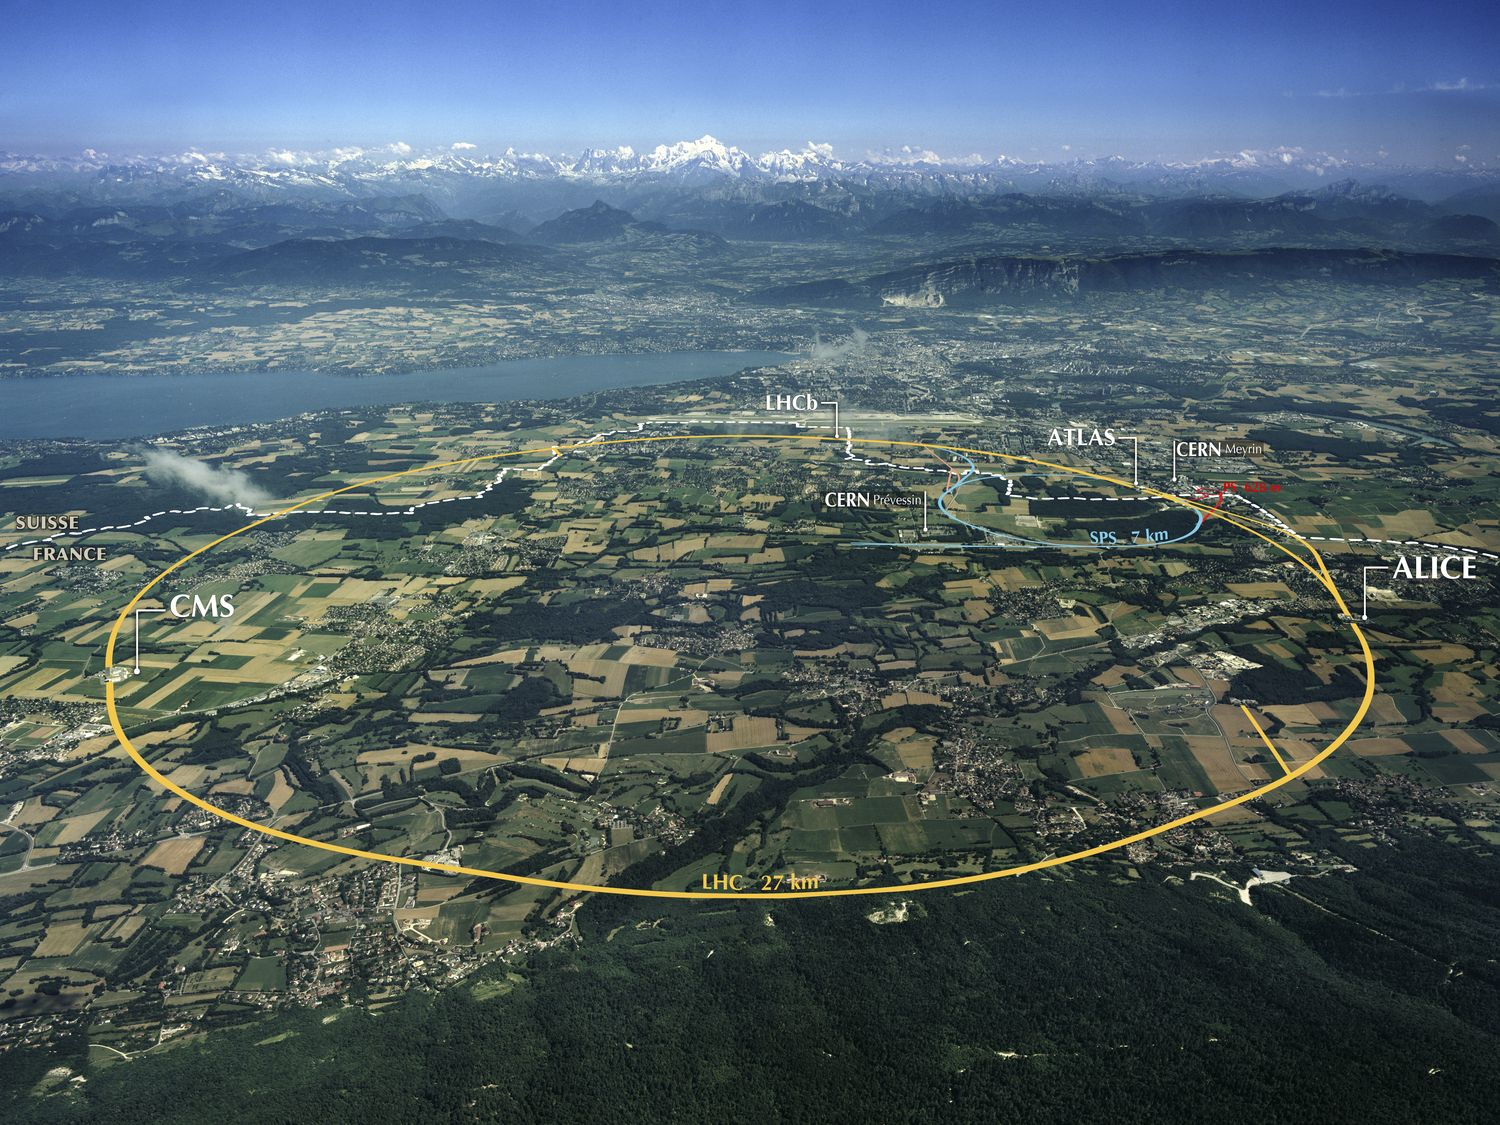
\includegraphics[width=0.4\textwidth]{figs/lhc.jpg}
\caption{The LHC complex; 17 miles around, 500ft underground.}
\label{fig:lhc}
\end{figure}
